\pdfminorversion=7
\DeclareUnicodeCharacter{2212}{-}
\documentclass{beamer}
\usepackage[utf8]{inputenc}
\usepackage{siunitx}
\usepackage{amsmath}
\usepackage{slashed}
\usepackage{fancyvrb}
\usepackage{epstopdf}
\usepackage{xcolor}
\hypersetup{
    colorlinks=true,
    linkcolor=blue,
    filecolor=magenta,      
    urlcolor=cyan,
}
\usetheme{boxes}
\newcommand{\ks}{\ensuremath{K_S^0}}
\newcommand{\strphdiff}{\ensuremath{\Delta \delta_D}}
\newcommand{\kspipi}[1]{\ensuremath{#1 \to \ks \pi^+ \pi^-}}
\newcommand{\diffDtokspipi}{\ensuremath{\kspipi{D^0}} \text{and} \ensuremath{\kspipi{\bar{D}^0}} }
\newcommand{\MP}{\ensuremath{m^2_+}}
\newcommand{\MM}{\ensuremath{m^2_-}}
\newcommand{\MZ}{\ensuremath{m^2_0}}
\newcommand{\phasePosition}{\ensuremath{m^2_+,m^2_-}}
\newcommand{\phasePositionT}{\ensuremath{m^2_-,m^2_+}}
\newcommand{\Dzbar}{\ensuremath{\bar{D}^0} }
\newcommand{\Dz}{\ensuremath{D^0} }
\newcommand{\Bzbar}{\ensuremath{\bar{B}^0} }
\newcommand{\Bz}{\ensuremath{B^0} }
%These macros are save time, usage
%\subAmp{particle}{component} -e.g \subAmp{\Dz}{L_{\pi^+\pi^-}=0}
\newcommand{\subAmp}[2]{\ensuremath{A_{#1}^{#2}\left(\phasePosition \right)}}
%\modelAmp{particle}{model name} - e.g. \modelAmp{\Dz}{Belle}
\newcommand{\modelAmp}[2]{\ensuremath{A_{#1}^{\text{#2}}\left(\phasePosition \right)}}
\newcommand{\genAmp}[2]{\ensuremath{A_{#1}^{\text{#2}}\left(\mathcal{P} \right)}}
%Generic input amp (actually you could use \modelAmp instead if you want
\newcommand{\inputAmp}[1]{\ensuremath{A_{#1}^{\text{input}}\left(\phasePosition\right)}}
%True model - what the decay really is
\newcommand{\trueAmp}[1]{\ensuremath{A_{#1}^{\text{True}}\left(\phasePosition\right)}}
%a_r and phi_r, again saves writing $, _, ^ everywhere
\newcommand{\magPar}[1]{\ensuremath{a_{#1}}}
\newcommand{\phPar}[1]{\ensuremath{\phi_{#1}}}
\author{Jake Lane}
\title{Implementation of the Belle Model for \diffDtokspipi decay in ampGen}
\begin{document}
\begin{frame}{}
    \maketitle
\end{frame}
\begin{frame}{Belle in Cartesian}
\begin{tiny}
\VerbatimInput{opts/Belle_in_Cartesian.opt}
\end{tiny}
\end{frame}
\begin{frame}{Belle in Cartesian}
\begin{figure}
\includegraphics[width=.8\linewidth]{Belle_in_Cartesian/Delta_gAbs.eps}
\caption{$\left|\frac{\genAmp{\Dz}{}}{\genAmp{\Dz}{}}\right|$ for Belle in Cartesian}
\end{figure}
\end{frame}
\begin{frame}{Belle in Cartesian}
\begin{figure}
\includegraphics[width=.8\linewidth]{Belle_in_Cartesian/Delta_gArg.eps}
\caption{\strphdiff for Belle in Cartesian}
\end{figure}
\end{frame}
\begin{frame}{Belle in Cartesian}
\begin{figure}
\includegraphics[width=.8\linewidth]{Belle_in_Cartesian/1D0/gArg.eps}
\caption{Argument for Belle in Cartesian}
\end{figure}
\end{frame}
\begin{frame}{Belle in Cartesian}
\begin{figure}
\includegraphics[width=.8\linewidth]{Belle_in_Cartesian/1D0/gAbs.eps}
\caption{Magnitude for Belle in Cartesian}
\end{figure}
\end{frame}
\begin{frame}{Belle in Cartesian}
\begin{figure}
\includegraphics[width=.8\linewidth]{Belle_in_Cartesian/1D0/s01.eps}
\caption{\MP for Belle in Cartesian}
\end{figure}
\end{frame}
\begin{frame}{Belle in Cartesian}
\begin{figure}
\includegraphics[width=.8\linewidth]{Belle_in_Cartesian/1D0/s02.eps}
\caption{\MM for Belle in Cartesian}
\end{figure}
\end{frame}
\begin{frame}{Belle in Cartesian}
\begin{figure}
\includegraphics[width=.8\linewidth]{Belle_in_Cartesian/1D0/s12.eps}
\caption{\MZ for Belle in Cartesian}
\end{figure}
\end{frame}
\begin{frame}{Belle in Cartesian}
\begin{figure}
\includegraphics[width=.8\linewidth]{Belle_in_Cartesian/1D0/s01_vs_s02.eps}
\caption{\MP vs \MM for Belle in Cartesian}
\end{figure}
\end{frame}
\begin{frame}{Belle in Cartesian}
\begin{figure}
\includegraphics[width=.8\linewidth]{Belle_in_Cartesian/1D0/s01_vs_s12.eps}
\caption{\MP vs \MZ for Belle in Cartesian}
\end{figure}
\end{frame}
\begin{frame}{Belle in Cartesian}
\begin{figure}
\includegraphics[width=.8\linewidth]{Belle_in_Cartesian/1D0/s02_vs_s12.eps}
\caption{\MP vs \MZ for Belle in Cartesian}
\end{figure}
\end{frame}

\begin{frame}{Belle in Cartesian}
\begin{figure}
\includegraphics[width=.8\linewidth]{Belle_in_Cartesian/1CCDbar0/gArg.eps}
\caption{Argument for Belle in Cartesian}
\end{figure}
\end{frame}
\begin{frame}{Belle in Cartesian}
\begin{figure}
\includegraphics[width=.8\linewidth]{Belle_in_Cartesian/1CCDbar0/gAbs.eps}
\caption{Magnitude for Belle in Cartesian}
\end{figure}
\end{frame}
\begin{frame}{Belle in Cartesian}
\begin{figure}
\includegraphics[width=.8\linewidth]{Belle_in_Cartesian/1CCDbar0/s01.eps}
\caption{\MP for Belle in Cartesian}
\end{figure}
\end{frame}
\begin{frame}{Belle in Cartesian}
\begin{figure}
\includegraphics[width=.8\linewidth]{Belle_in_Cartesian/1CCDbar0/s02.eps}
\caption{\MM for Belle in Cartesian}
\end{figure}
\end{frame}
\begin{frame}{Belle in Cartesian}
\begin{figure}
\includegraphics[width=.8\linewidth]{Belle_in_Cartesian/1CCDbar0/s12.eps}
\caption{\MZ for Belle in Cartesian}
\end{figure}
\end{frame}
\begin{frame}{Belle in Cartesian}
\begin{figure}
\includegraphics[width=.8\linewidth]{Belle_in_Cartesian/1CCDbar0/s01_vs_s02.eps}
\caption{\MP vs \MM for Belle in Cartesian}
\end{figure}
\end{frame}
\begin{frame}{Belle in Cartesian}
\begin{figure}
\includegraphics[width=.8\linewidth]{Belle_in_Cartesian/1CCDbar0/s01_vs_s12.eps}
\caption{\MP vs \MZ for Belle in Cartesian}
\end{figure}
\end{frame}
\begin{frame}{Belle in Cartesian}
\begin{figure}
\includegraphics[width=.8\linewidth]{Belle_in_Cartesian/1CCDbar0/s02_vs_s12.eps}
\caption{\MP vs \MZ for Belle in Cartesian}
\end{figure}
\end{frame}


\begin{frame}{Belle in Polar}
\begin{tiny}
\VerbatimInput{opts/Belle_in_Polar.opt}
\end{tiny}
\end{frame}
\begin{frame}{Belle in Polar}
\begin{figure}
\includegraphics[width=.8\linewidth]{Belle_in_Polar/Delta_gAbs.eps}
\caption{$\left|\frac{\genAmp{\Dz}{}}{\genAmp{\Dz}{}}\right|$ for Belle in Polar}
\end{figure}
\end{frame}
\begin{frame}{Belle in Polar}
\begin{figure}
\includegraphics[width=.8\linewidth]{Belle_in_Polar/Delta_gArg.eps}
\caption{\strphdiff for Belle in Polar}
\end{figure}
\end{frame}
\begin{frame}{Belle in Polar}
\begin{figure}
\includegraphics[width=.8\linewidth]{Belle_in_Polar/1D0/gArg.eps}
\caption{Argument for Belle in Polar}
\end{figure}
\end{frame}
\begin{frame}{Belle in Polar}
\begin{figure}
\includegraphics[width=.8\linewidth]{Belle_in_Polar/1D0/gAbs.eps}
\caption{Magnitude for Belle in Polar}
\end{figure}
\end{frame}
\begin{frame}{Belle in Polar}
\begin{figure}
\includegraphics[width=.8\linewidth]{Belle_in_Polar/1D0/s01.eps}
\caption{\MP for Belle in Polar}
\end{figure}
\end{frame}
\begin{frame}{Belle in Polar}
\begin{figure}
\includegraphics[width=.8\linewidth]{Belle_in_Polar/1D0/s02.eps}
\caption{\MM for Belle in Polar}
\end{figure}
\end{frame}
\begin{frame}{Belle in Polar}
\begin{figure}
\includegraphics[width=.8\linewidth]{Belle_in_Polar/1D0/s12.eps}
\caption{\MZ for Belle in Polar}
\end{figure}
\end{frame}
\begin{frame}{Belle in Polar}
\begin{figure}
\includegraphics[width=.8\linewidth]{Belle_in_Polar/1D0/s01_vs_s02.eps}
\caption{\MP vs \MM for Belle in Polar}
\end{figure}
\end{frame}
\begin{frame}{Belle in Polar}
\begin{figure}
\includegraphics[width=.8\linewidth]{Belle_in_Polar/1D0/s01_vs_s12.eps}
\caption{\MP vs \MZ for Belle in Polar}
\end{figure}
\end{frame}
\begin{frame}{Belle in Polar}
\begin{figure}
\includegraphics[width=.8\linewidth]{Belle_in_Polar/1D0/s02_vs_s12.eps}
\caption{\MP vs \MZ for Belle in Polar}
\end{figure}
\end{frame}

\begin{frame}{Belle in Polar}
\begin{figure}
\includegraphics[width=.8\linewidth]{Belle_in_Polar/1CCDbar0/gArg.eps}
\caption{Argument for Belle in Polar}
\end{figure}
\end{frame}
\begin{frame}{Belle in Polar}
\begin{figure}
\includegraphics[width=.8\linewidth]{Belle_in_Polar/1CCDbar0/gAbs.eps}
\caption{Magnitude for Belle in Polar}
\end{figure}
\end{frame}
\begin{frame}{Belle in Polar}
\begin{figure}
\includegraphics[width=.8\linewidth]{Belle_in_Polar/1CCDbar0/s01.eps}
\caption{\MP for Belle in Polar}
\end{figure}
\end{frame}
\begin{frame}{Belle in Polar}
\begin{figure}
\includegraphics[width=.8\linewidth]{Belle_in_Polar/1CCDbar0/s02.eps}
\caption{\MM for Belle in Polar}
\end{figure}
\end{frame}
\begin{frame}{Belle in Polar}
\begin{figure}
\includegraphics[width=.8\linewidth]{Belle_in_Polar/1CCDbar0/s12.eps}
\caption{\MZ for Belle in Polar}
\end{figure}
\end{frame}
\begin{frame}{Belle in Polar}
\begin{figure}
\includegraphics[width=.8\linewidth]{Belle_in_Polar/1CCDbar0/s01_vs_s02.eps}
\caption{\MP vs \MM for Belle in Polar}
\end{figure}
\end{frame}
\begin{frame}{Belle in Polar}
\begin{figure}
\includegraphics[width=.8\linewidth]{Belle_in_Polar/1CCDbar0/s01_vs_s12.eps}
\caption{\MP vs \MZ for Belle in Polar}
\end{figure}
\end{frame}
\begin{frame}{Belle in Polar}
\begin{figure}
\includegraphics[width=.8\linewidth]{Belle_in_Polar/1CCDbar0/s02_vs_s12.eps}
\caption{\MP vs \MZ for Belle in Polar}
\end{figure}
\end{frame}


\begin{frame}{Belle in Polar times Fit Fractions}
\begin{tiny}
\VerbatimInput{opts/Belle_in_Polar_times_Fit_Fractions.opt}
\end{tiny}
\end{frame}
\begin{frame}{Belle in Polar times Fit Fractions}
\begin{figure}
\includegraphics[width=.8\linewidth]{Belle_in_Polar_times_Fit_Fractions/Delta_gAbs.eps}
\caption{$\left|\frac{\genAmp{\Dz}{}}{\genAmp{\Dz}{}}\right|$ for Belle in Polar times Fit Fractions}
\end{figure}
\end{frame}
\begin{frame}{Belle in Polar times Fit Fractions}
\begin{figure}
\includegraphics[width=.8\linewidth]{Belle_in_Polar_times_Fit_Fractions/Delta_gArg.eps}
\caption{\strphdiff for Belle in Polar times Fit Fractions}
\end{figure}
\end{frame}
\begin{frame}{Belle in Polar times Fit Fractions}
\begin{figure}
\includegraphics[width=.8\linewidth]{Belle_in_Polar_times_Fit_Fractions/1D0/gArg.eps}
\caption{Argument for Belle in Polar times Fit Fractions}
\end{figure}
\end{frame}
\begin{frame}{Belle in Polar times Fit Fractions}
\begin{figure}
\includegraphics[width=.8\linewidth]{Belle_in_Polar_times_Fit_Fractions/1D0/gAbs.eps}
\caption{Magnitude for Belle in Polar times Fit Fractions}
\end{figure}
\end{frame}
\begin{frame}{Belle in Polar times Fit Fractions}
\begin{figure}
\includegraphics[width=.8\linewidth]{Belle_in_Polar_times_Fit_Fractions/1D0/s01.eps}
\caption{\MP for Belle in Polar times Fit Fractions}
\end{figure}
\end{frame}
\begin{frame}{Belle in Polar times Fit Fractions}
\begin{figure}
\includegraphics[width=.8\linewidth]{Belle_in_Polar_times_Fit_Fractions/1D0/s02.eps}
\caption{\MM for Belle in Polar times Fit Fractions}
\end{figure}
\end{frame}
\begin{frame}{Belle in Polar times Fit Fractions}
\begin{figure}
\includegraphics[width=.8\linewidth]{Belle_in_Polar_times_Fit_Fractions/1D0/s12.eps}
\caption{\MZ for Belle in Polar times Fit Fractions}
\end{figure}
\end{frame}
\begin{frame}{Belle in Polar times Fit Fractions}
\begin{figure}
\includegraphics[width=.8\linewidth]{Belle_in_Polar_times_Fit_Fractions/1D0/s01_vs_s02.eps}
\caption{\MP vs \MM for Belle in Polar times Fit Fractions}
\end{figure}
\end{frame}
\begin{frame}{Belle in Polar times Fit Fractions}
\begin{figure}
\includegraphics[width=.8\linewidth]{Belle_in_Polar_times_Fit_Fractions/1D0/s01_vs_s12.eps}
\caption{\MP vs \MZ for Belle in Polar times Fit Fractions}
\end{figure}
\end{frame}
\begin{frame}{Belle in Polar times Fit Fractions}
\begin{figure}
\includegraphics[width=.8\linewidth]{Belle_in_Polar_times_Fit_Fractions/1D0/s02_vs_s12.eps}
\caption{\MP vs \MZ for Belle in Polar times Fit Fractions}
\end{figure}
\end{frame}

\begin{frame}{Belle in Polar times Fit Fractions}
\begin{figure}
\includegraphics[width=.8\linewidth]{Belle_in_Polar_times_Fit_Fractions/1CCDbar0/gArg.eps}
\caption{Argument for Belle in Polar times Fit Fractions}
\end{figure}
\end{frame}
\begin{frame}{Belle in Polar times Fit Fractions}
\begin{figure}
\includegraphics[width=.8\linewidth]{Belle_in_Polar_times_Fit_Fractions/1CCDbar0/gAbs.eps}
\caption{Magnitude for Belle in Polar times Fit Fractions}
\end{figure}
\end{frame}
\begin{frame}{Belle in Polar times Fit Fractions}
\begin{figure}
\includegraphics[width=.8\linewidth]{Belle_in_Polar_times_Fit_Fractions/1CCDbar0/s01.eps}
\caption{\MP for Belle in Polar times Fit Fractions}
\end{figure}
\end{frame}
\begin{frame}{Belle in Polar times Fit Fractions}
\begin{figure}
\includegraphics[width=.8\linewidth]{Belle_in_Polar_times_Fit_Fractions/1CCDbar0/s02.eps}
\caption{\MM for Belle in Polar times Fit Fractions}
\end{figure}
\end{frame}
\begin{frame}{Belle in Polar times Fit Fractions}
\begin{figure}
\includegraphics[width=.8\linewidth]{Belle_in_Polar_times_Fit_Fractions/1CCDbar0/s12.eps}
\caption{\MZ for Belle in Polar times Fit Fractions}
\end{figure}
\end{frame}
\begin{frame}{Belle in Polar times Fit Fractions}
\begin{figure}
\includegraphics[width=.8\linewidth]{Belle_in_Polar_times_Fit_Fractions/1CCDbar0/s01_vs_s02.eps}
\caption{\MP vs \MM for Belle in Polar times Fit Fractions}
\end{figure}
\end{frame}
\begin{frame}{Belle in Polar times Fit Fractions}
\begin{figure}
\includegraphics[width=.8\linewidth]{Belle_in_Polar_times_Fit_Fractions/1CCDbar0/s01_vs_s12.eps}
\caption{\MP vs \MZ for Belle in Polar times Fit Fractions}
\end{figure}
\end{frame}
\begin{frame}{Belle in Polar times Fit Fractions}
\begin{figure}
\includegraphics[width=.8\linewidth]{Belle_in_Polar_times_Fit_Fractions/1CCDbar0/s02_vs_s12.eps}
\caption{\MP vs \MZ for Belle in Polar times Fit Fractions}
\end{figure}
\end{frame}


\begin{frame}{To Do}
\begin{itemize}
\item Cartesian times Fit Fraction
\item Convert any model (Belle, BaBar) to Re,Im (use excel?)
\item Fitting is also done in Re-Im, it might be an ampGen error?
\end{itemize}
\end{frame}
\end{document}
